\newpage
\section{Appendix}
\label{Appendix}

We provide proofs for our theoretical results (App. \ref{app:proofs}), an algorithm block detailing our method (App. \ref{app:algorithm}), and additional experiments and experimental details (App. \ref{app:parameters}).
\subsection{Proofs}\label{app:proofs}
\setcounter{theorem}{0}
\begin{lemma}[KRS overapproximation]
\label{lem:koopman_containment}
Let $\tnfl$ denote the closed-loop CG of TKFL, and let $\mathcal{X}_0$ be the initial set. Suppose the KRS $\hat{\overline{\mathcal{X}}}_{0:T}$ is defined as in \eqref{eq:Koopman_RSOA}. Then, for any initial state $x_0 \in \mathcal{X}_0$, the decoded closed-loop trajectory \eqref{eq:latent_rollout_tnfl}, i.e., 
$\hat{x}_{0:T} = \tnfl(x_0, \zref_{0:T}, \uref_{0:T-1})$ satisfies $\hat{x}_t \in \hat{\mathcal{X}}_t$ for all $t \in \mathcal{T}$.
\end{lemma}

\begin{proof}
The closed-loop graph $\tnfl$ is a computational graph $G$ as defined in Proposition~\ref{thm:cg_robustness}. Using the \texttt{auto\_LiRPA} library~\cite{Xu2020AutoLiRPA}, we compute sound, vector-valued affine bounding functions $\underline{\tnfl}_t$ and $\overline{\tnfl}_t$ (corresponding to $\underline{G}$ and $\overline{G}$ in Proposition~\ref{thm:cg_robustness}) for the $t$-th state output.

By Proposition~\ref{thm:cg_robustness}, these bounds are guaranteed to be sound. That is, for any specific input $x_0 \in \mathcal{X}_0$, the predicted state 
$\hat{x}_t = \tnfl_t(x_0, \zref_{0:T}, \uref_{0:T-1})$ satisfies
\[
\underline{\tnfl}_t(x_0, \zref_{0:T}, \uref_{0:T-1}) 
\le \hat{x}_t 
\le \overline{\tnfl}_t(x_0, \zref_{0:T}, \uref_{0:T-1}).
\]

The KRS $\hat{\overline{\mathcal{X}}}_t$ is defined in \eqref{eq:Koopman_RSOA} as the interval $\textsf{Int}(\hat{x}_t^L, \hat{x}_t^U)$, where $\hat{x}_t^L = \min_{x_0' \in \mathcal{X}_0} \underline{\tnfl}_t(x_0', \dots)$ and $\hat{x}_t^U = \max_{x_0' \in \mathcal{X}_0} \overline{\tnfl}_t(x_0', \dots)$.
By the definitions of the minimum and maximum, we have
\begin{align*}
    \hat{x}_t 
    &\ge \underline{\tnfl}_t(x_0, \dots) 
     \ge \min_{x_0' \in \mathcal{X}_0} \underline{\tnfl}_t(x_0', \dots) 
     = \hat{x}_t^L,\\
    \hat{x}_t 
    &\le \overline{\tnfl}_t(x_0, \dots) 
     \le \max_{x_0' \in \mathcal{X}_0} \overline{\tnfl}_t(x_0', \dots) 
     = \hat{x}_t^U.
\end{align*}
Hence, $\hat{x}_t \in \textsf{Int}(\hat{x}_t^L, \hat{x}_t^U) = \hat{\overline{\mathcal{X}}}_t$. Since this holds for all $t \in \mathcal{T}$, the trajectory $\hat{x}_{0:T}$ is contained within $\hat{\overline{\mathcal{X}}}_{0:T}$.
\end{proof}

\setcounter{theorem}{0}
\begin{theorem}[CKRS Coverage Guarantee]
\label{thm:ckrs_coverage}
Let $\hat{\overline{\mathcal{X}}}_{0:T}$ be the KRS defined in \eqref{eq:Koopman_RSOA} and let $\bar e_t = [\bar e_{t,1}, \ldots, \bar e_{t,n}]^\top \in \mathbb{R}^n$. Define the conformalized Koopman reachable set (CKRS) as
\begin{equation}
\overline{\mathcal{X}}_{0:T}^{1-\delta} \equiv \bigl\{ \hat{\overline{\mathcal{X}}}_t \oplus \mathrm{diag}(\bar e_t) \mathcal{B}_1(0) \bigr\}_{t=0}^T,
\label{eq:conformal_inflation}
\end{equation}
where $\mathrm{diag}(\bar e_t) \in \mathbb{R}^{n\times n}$ is a diagonal matrix with $\bar e_t$ on its diagonal. Then, for a new reference trajectory $x_{0:T}^{\textrm{ref}, (0)}$ drawn from the same distribution, the CKRS contains true closed-loop system trajectory generated by \eqref{eq:closed_loop_dynamics} with probability at least $1-\delta$:
\[
\mathbb{P}\Big( \bigwedge_{t=0}^T x_t^{(0)} \in \overline{\mathcal{X}}_t^{1-\delta} \Big) \ge 1-\delta.
\]
\end{theorem}

\begin{proof}
The proof combines a deterministic containment guarantee with a probabilistic coverage guarantee.

\noindent\textit{Step 1: KRS Containment.}  
By Lemma~\ref{lem:koopman_containment}, the decoded closed-loop lifted trajectory $\hat{x}_{t,j}^{(0)}$ is deterministically contained within the hyper-rectangular KRS:
\[
\hat{x}_{t,j}^{(0)} \in \hat{\overline{\mathcal{X}}}_{t,j} = \textsf{Int}(\hat{x}_{t,j}^L, \hat{x}_{t,j}^U), \quad \forall t \in \mathcal{T},\quad \forall j \in \{1,\ldots,n\}.
\]

\noindent\textit{Step 2: Probabilistic Coverage.}  
The CP guarantee requires exchangeability of the nonconformity scores $\{\ncscore^{(i)}\}_{i=0}^{K^{\mathrm{cal}}}$. In our framework, all calibration and test trajectories share the same reference $(z_{0:T}^{\mathrm{ref}}, u_{0:T-1}^{\mathrm{ref}})$ and controller $\lqrmat_t$, and their initial states $x_0^{(i)}$ are sampled i.i.d. from $\mathcal{B}_\epsilon(x_0^{\mathrm{ref}})$. Since the decoded closed-loop lifted trajectory \eqref{eq:latent_rollout}, true closed-loop trajectory \eqref{eq:actual_rollout}, and the nonconformity score are deterministic functions of $x_0^{(i)}$, the resulting scores $\ncscore^{(i)}$ are also i.i.d., and hence exchangeable. By the CP guarantee, the event
\[
\mathcal{E} \equiv \{ |e_{t,j}^{(0)}| \le \bar e_{t,j}, \forall t,j \}
\]
occurs with probability at least $1-\delta$.

\noindent\textit{Step 3: Combined Guarantee.}  
The true state can be decomposed as $x_{t,j}^{(0)} = \hat{x}_{t,j}^{(0)} + e_{t,j}^{(0)}$. When $\mathcal{E}$ occurs, we have
\[
\hat{x}_{t,j}^L - \bar e_{t,j} \le \hat{x}_{t,j}^{(0)} + e_{t,j}^{(0)} \le \hat{x}_{t,j}^U + \bar e_{t,j},
\]
which by definition implies $x_{t,j}^{(0)} \in \overline{\mathcal{X}}_{t,j}^{1-\delta}$. Since this holds for all $t$ and $j$, the trajectory $x_{0:T}^{(0)}$ is contained in the CKRS $\overline{\mathcal{X}}_{0:T}^{1-\delta}$ with probability at least $1-\delta$.
\end{proof}

\subsection{Algorithm}\label{app:algorithm}

Algorithm \ref{alg:online_ckrs} details the procedure for computing the CKRS. The process begins by lifting the planner-provided reference trajectory $x_{0:T}^\textrm{ref}$ into the latent space to compute the feedforward control $u^\textrm{ref}$ via least-squares, and synthesizing a time-varying LQR controller to track this reference. To account for the discrepancy between the learned Koopman dynamics and the true system, the algorithm generates calibration data from system rollouts and utilizes SNSA-based conformal prediction to derive statistically-valid error bounds $\bar e_t$. In parallel, the nominal KRS, $\overline{\mathcal{X}}_{0:T}$, is computed by constructing a computational graph of the closed-loop tracking dynamics in the lifted Koopman state space and computing reachable sets for the linear Koopman dynamics via \texttt{auto\_LiRPA}. Finally, the algorithm returns a conformalized Koopman reachable set (CKRS), $\mathcal{X}_{0:T}^{1-\delta}$, obtained by inflating the nominal KRS with the derived conformal error bounds via a Minkowski sum. Crucially, the CKRS guarantees coverage of the trajectories generated by the \textit{true system} with probability $1-\delta$.

\begin{algorithm}[]

\caption{Online Conformalized Koopman Reachable Set (CKRS)}
\label{alg:online_ckrs}
\begin{algorithmic}[1]
 \Require Koopman model ($\enc, \dec, \ka, \kb$); true dynamics $f$ (simulator); reference trajectory $x^{\text{ref}}_{0:T}$; initial set $\mathcal{X}_0 = \mathcal{B}_\epsilon(x_0^{\text{ref}})$; RSOA confidence $1-\delta$; calibration sizes $M^{\lambda}, K^{\text{cal}}$; cost matrices $Q, R$; verification tool $\texttt{auto\_LiRPA}$
 \Ensure Conformalized Koopman reachable set $\overline{\mathcal{X}}^{1-\delta}_{0:T}$ (CKRS)
 \Statex \Comment{1. Initialization}
 \State $z^{\text{ref}}_{0:T} \gets \enc(x^{\text{ref}}_{0:T})$ \Comment{encode reference state trajectory}
 \State $u^{\text{ref}}_{0:T-1} \gets$ Equation \eqref{eq:u_ff} \Comment{compute feedforward control sequence}
 \State $\lqrmat_{0:T-1} \gets$ \textrm{LQR}$(K_A, K_B)$ \Comment{compute LQR gains}
 \State $\pi(\cdot) \gets$ Equation \eqref{eq:u_latent_cl} \Comment{compute lifted controller using LQR and feedforward inputs}
 \Statex \Comment{2. Error bounds $\bar e_t$ via CP}
 \State $\mathcal{D}_E, \mathcal{D}_N \gets \texttt{GenerateCalibrationData}(M^{\lambda}, K^{\text{cal}})$
 \State $\bar e_t \gets \texttt{SNSA}(\mathcal{D}_N, \mathcal{D}_E)$
 \Statex \Comment{3. Nominal KRS $\hat{\overline{\mathcal{X}}}_{0:T}$}
 \State $\tnfl(\cdot) \gets \dec(\texttt{PropagateLatent}(\enc(\cdot), z^{\text{ref}}, u^{\text{ref}}, \lqrmat))$ \Comment{define CG}
 \State $\hat{\overline{\mathcal{X}}}_{0:T} \gets \texttt{AutoLiRPA}(\tnfl, \mathcal{X}_0)$ \Comment{compute KRS via CG}
 \State $\overline{\mathcal{X}}^{1-\delta}_{0:T} \gets \hat{\overline{\mathcal{X}}}_{0:T} \oplus \textrm{diag}(\bar e_t) \mathcal{B}_1(0)$ \Comment{4. combine to obtain CKRS, and return}
 \State \textbf{return} $\overline{\mathcal{X}}^{1-\delta}_{0:T}$
\end{algorithmic}
\end{algorithm}


\subsection{Experiment Details and Additional Experiments}\label{app:parameters}

The following section contains the the analytical dynamics we used in this paper (App. \ref{app:dynamics}) and additional experiment results. In particular, we benchmark our approach with a baseline Koopman dynamics learning approach that leverages polynomial liftings (App. \ref{app:polynomial}), a baseline learned reachable set prediction method (App. \ref{app:deepreach}), and a baseline conformal prediction-based reachable set computation method that does not leverage Koopman-based propagation (App. \ref{app:nnv}). We also present additional experiment figures, including full reachable set visualizations on a per-state breakdown for the unicycle system (App. \ref{app:unicycle}), planar quadcopter system (App. \ref{app:quadcopter}), MuJoCo hopper system (App. \ref{app:hopper}), and MuJoCo swimmer system (App. \ref{app:swimmer}).

\subsubsection{Dynamics. }\label{app:dynamics}
For unicycle experiments ($x \in \mathbb{R}^3$, $u \in \mathbb{R}^2$), we used the dynamics model, time-discretized via forward Euler ($dt =0.1$s)
\begin{equation}\label{eq:unicycle}
    \dot{\mathbf{x}}\;=\; f(\mathbf{x},\mathbf{u})=
    \begin{bmatrix}
        u_1 \cos(x_2) \\ u_1 \sin(x_2) \\ u_2
    \end{bmatrix}.
\end{equation}

\noindent For planar quadcopter experiments ($x \in \mathbb{R}^6$, $u \in \mathbb{R}^2$), we used the parameters $m=0.5\textrm{kg}$, $g=-9.81\textrm{m/s}^2$, $I_y=0.01\textrm{kg} \cdot \textrm{m}^2$ for the dynamics model, and time-discretized with $dt = 0.05\,\mathrm{s}$:%. The result are shown in Fig. \ref{fig:2d_quad}:
\begin{equation}\label{eq:2dquad}
    \dot{\mathbf{x}}\;=\; f(\mathbf{x},\mathbf{u})=\begin{bmatrix}
        x_4 \\ x_5 \\ x_6 \\ -\frac{u_1}{m} \sin(x_3)\\ g+\frac{u_1}{m}\cos(x_3)\\\frac{u_2}{I_y}
    \end{bmatrix}
\end{equation}

\noindent For 3D quadcopter experiments, we used the parameters $m=1$kg, $g=-9.81$ m/s$^2$, $I_{x,y,z}=[0.5,0.1,0.3]$ kg·m$^2$ for the dynamics, with a time-discretization of $dt = 0.025\,\mathrm{s}$:
\begin{equation}
    \dot{\mathbf{x}} \;=\; f(\mathbf{x},\mathbf{u})=
    \begin{bmatrix}
        \dot{x} \\
        \dot{y} \\
        \dot{z} \\
        q \cdot \sin(\phi)/\cos{\theta}+r\cdot \cos{\phi}/\cos{\theta} \\
        q \cdot \cos{\phi} - r\cdot \sin{\phi} \\
        p + q \cdot \sin{\phi}\cdot \tan{\theta} +r\cdot \cos{\phi} \cdot \tan{\theta} \\
        \frac{u_1}{m} \cdot (\sin{\phi} \cdot \sin{\psi} + \cos{\phi} \cdot \cos{\psi} \cdot \sin{\theta}) \\ 
        \frac{u_1}{m} \cdot (\cos{\phi} \cdot \sin{\phi} - \cos{\phi} \cdot \sin{\psi} \cdot \sin{\theta}) \\ 
        g + u_1 \cdot (\cos{\phi} \cdot \cos{\theta}) / m\\
        ((I_y - I_z) / I_x) \cdot q\cdot r + \frac{u_2}{I_x} \\
        ((I_z - I_x) / I_y) \cdot p\cdot r + \frac{u_3}{I_y} \\
        ((I_x - I_y) / I_z) \cdot p\cdot q + \frac{u_4}{I_z} \\
    \end{bmatrix}
    \label{eq:3D_Quad_dyn}
\end{equation}

\subsubsection{Comparison between neural Koopman liftings and polynomial liftings}\label{app:polynomial}
We compare root mean square error (RMSE) between a polynomial-lifted extended dynamic mode decomposition baseline and our neural lifting approach on the Hopper system. For the polynomial lift, we use PyKoopman \citep{pykoopman} with degree-3 monomials and identical training data/preprocessing. During open-loop evaluation, the polynomial model becomes numerically unstable, that is, its predictions grow without bound and diverge by the eighth timestep, so we report RMSE only over the first 5 prediction steps in Table \ref{tab:hopper_11d_rmse}. In contrast, our neural lifting yields a stable latent dynamics model that tracks accurately across three complete hops, enabling longer-horizon evaluation. These results highlight that for certain systems, e.g., those with strongly nonlinear, contact-rich dynamics (like the MuJoCo hopper), fixed polynomial bases are insufficient, whereas a neural network lifting function captures the necessary structure and remains stable over extended rollouts. Together, these results motivate the development of a Koopman reachable-set computation framework that incorporates neural networks in the loop, which we enable using \texttt{auto\_LiRPA}.

\begin{table}[ht]
\centering
\begin{tabular}{lrr}
\hline
\textbf{State} & \textbf{Polynomial Lifting} & \textbf{Ours} \\
\hline
z-coord (height)   & 2728.481591        & 0.009848 \\
torso angle        & 117.374908         & 0.004201 \\
thigh joint        & 2832.025934        & 0.013581 \\
leg joint          & 10791.162550       & 0.015690 \\
foot joint         & 8063.167273        & 0.017901 \\
vel x-coord        & 321013.541866      & 0.047526 \\
vel z-coord        & 1691803.060196     & 0.059763 \\
vel torso          & 4512148.680118     & 0.082879 \\
vel thigh          & 596074.452102      & 0.073777 \\
vel leg            & 6164730.041985     & 0.164258 \\
vel foot           & 135554800.971296   & 0.259034 \\
\hline
\end{tabular}
\caption{RMSE comparison for the hopper (11D) system on rollouts performed by the learned model and the polynomial fitted model.}
\label{tab:hopper_11d_rmse}
\end{table}

\subsubsection{Baseline comparison with \cite{deepreach}.}\label{app:deepreach}

Figure~\ref{fig:deepreach} offers a qualitative comparison of safety violations between the baseline DeepReach method \citep{deepreach} and ScaRe-Kro. While the main text statistics indicate a lower safety rate for the baseline, this visualization explicitly captures the ``reach-avoid" failure mode: the orange trajectories generated by the DeepReach value function clearly drift into the red obstacle region. This highlights the risks of relying on approximate neural PDE solutions for safety-critical constraints. In contrast, the reachable set (shown in blue) computed by our method creates a tight, verified corridor that contains the ground truth rollouts with high, calibrated probability, visually confirming that the controller successfully steers the dynamics clear of the hazard while adhering to the probabilistic bounds.

\begin{figure}[ht]
  \centering
  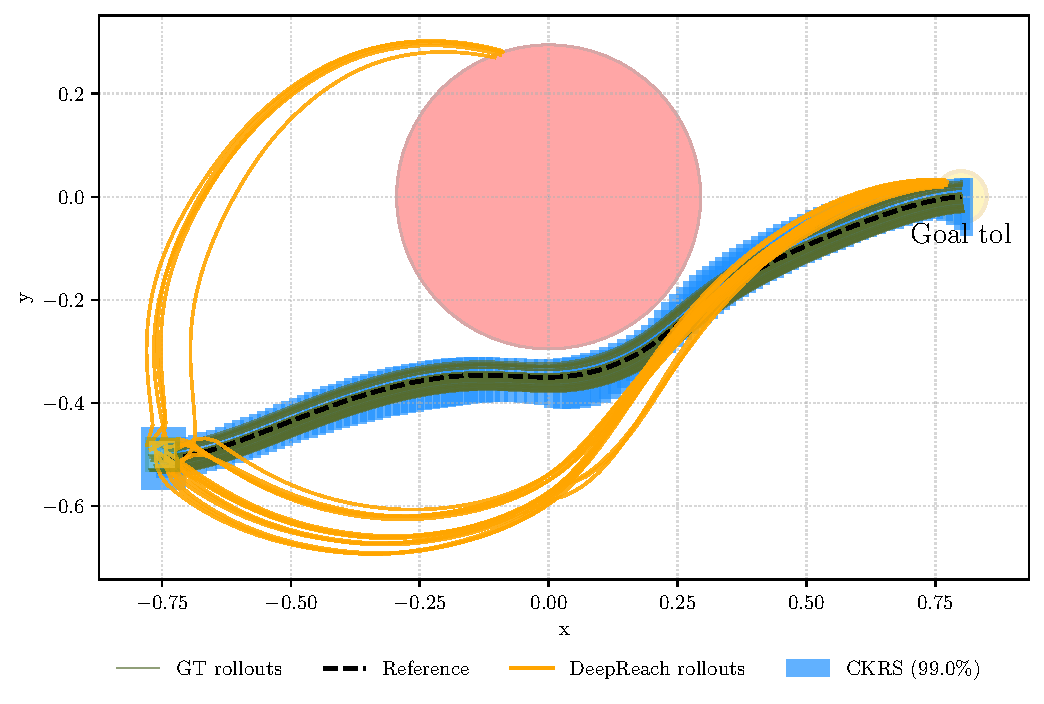
\includegraphics[width=1\linewidth]{img/baseline/deepreach.pdf}
  \caption{Closed-loop trajectories obtained from DeepReach-based controller (orange) can fail to enforce the reach-avoid constraint (reach yellow goal region while avoiding red unsafe set), while our controller (green rollouts) guarantees safety and containment within the blue CKRS with probability 0.99.}
  \label{fig:deepreach}
\end{figure}

\subsubsection{Baseline comparison with \cite{cp_baseline}.}\label{app:nnv}
Figure~\ref{fig:cpnnv} provides a state-by-state breakdown of the conservativeness gap between the reachable sets computed via the baseline CP-NNV \citep{cp_baseline} approach (yellow) and our proposed method (blue). While the tabular results in Section~\ref{sec:experiments} quantify the volume difference, Figure \ref{fig:cpnnv} illustrate where that difference originates visually. Overall, one of the key differences between our approach and \cite{cp_baseline} is in using a learned multi-step predictor instead of learned Koopman dynamics to compute reachable sets. We note that the CP-NNV method suffers from more conservative reachable sets, particularly in the angular velocity ($p, q, r$) and angle ($\phi, \theta, \psi$) dimensions. We attribute this to the difficulty of computing reachable sets accurately with a learned multi-step predictor over long horizons. Conversely, ScaRe-Kro maintains consistently tight bounds across all 12 dimensions, demonstrating that the Koopman linearization effectively mitigates the ``wrapping effect" that causes over-approximation in standard neural network verification.

\begin{figure}[ht]
    \centering
    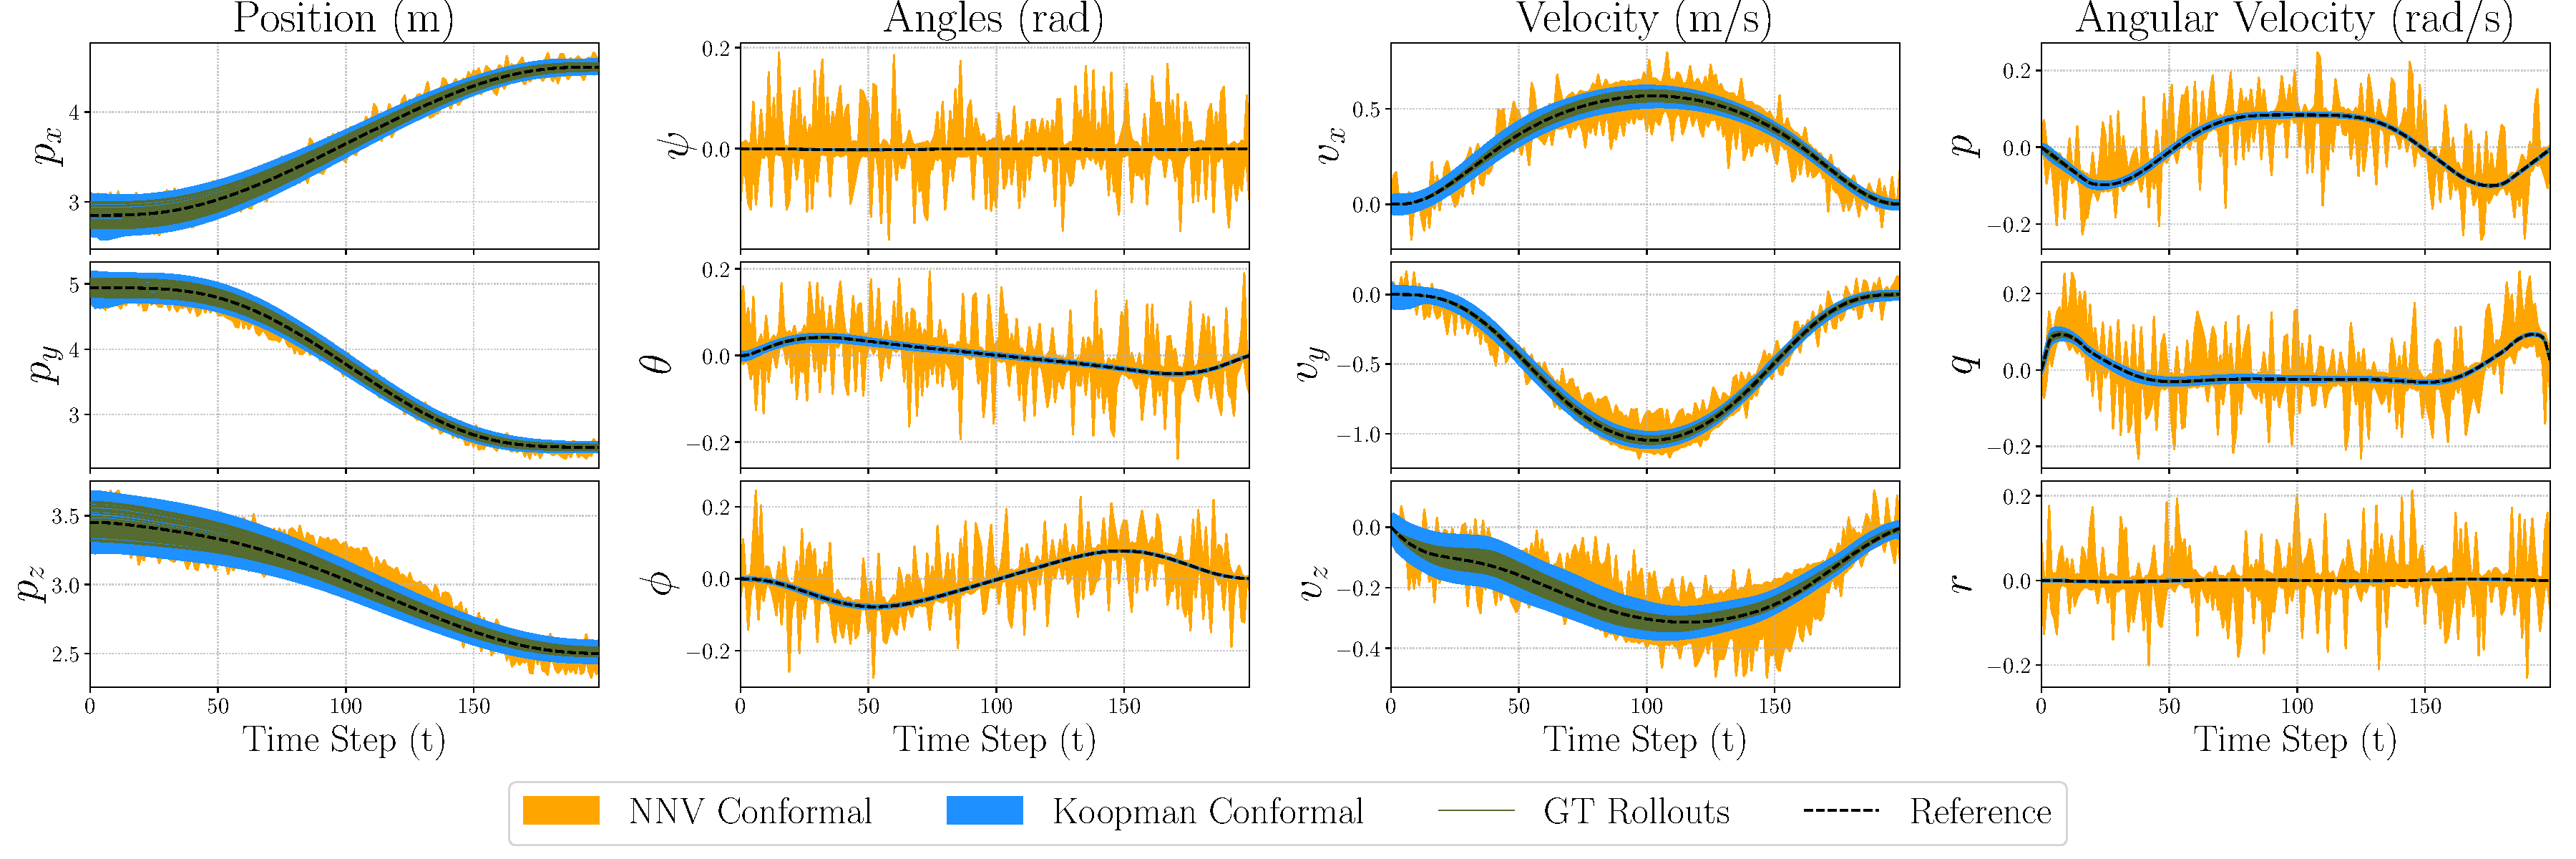
\includegraphics[width=1\linewidth]{img/baseline/NNV_Baseline.pdf}
    \caption{Baseline comparison between CP NNV approach and our method}
    \label{fig:cpnnv}
\end{figure}

\subsubsection{Additional results on unicycle system.}\label{app:unicycle}
Figure~\ref{fig:car} depicts the spatial evolution of the CKRS for the unicycle. Beyond the numerical coverage rates of Sec. \ref{sec:experiments}, this plot serves as a geometric sanity check, showing the reachable set's ability to contain the reference trajectory (black dashed line) and closed-loop trajectories (green) while navigating tight constraints. The blue tube is the CKRS that represents the region where the system is guaranteed to remain with with probability at least $1-\delta$, illustrating that even with the reachable set inflation induced by the conformalization step, the resulting set remains sufficiently compact to verify safety despite the closeness of the closed-loop rollouts to the red obstacle.

\begin{figure}[ht]
  \centering
  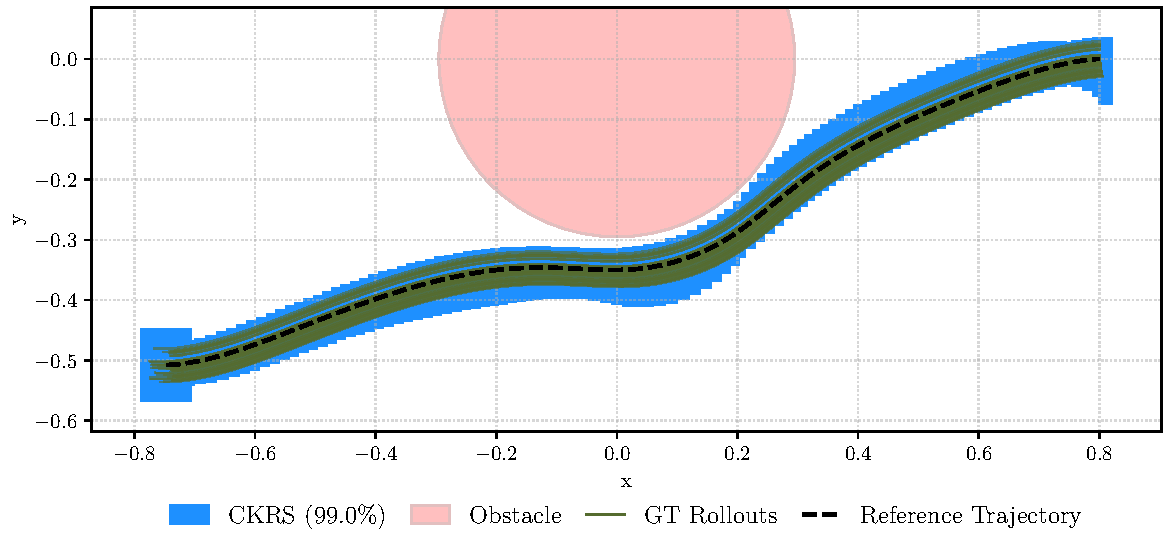
\includegraphics[width=1\linewidth]{img/car/car_frs_plot.pdf}
  \caption{CKRS computed for 3D unicycle model, enabling safety verification despite the small distance of the closed-loop trajectories to the obstacle (red).}
  \label{fig:car}
\end{figure}

\subsubsection{Additional results on planar quadcopter system.}\label{app:quadcopter}
We present the full dimensional trajectory evolution for the 6D planar quadcopter in Figure~\ref{fig:2d_quad}. These plots isolate the performance of the Koopman tracking controller on an underactuated system. Notably, the reachable sets (light blue) and their conformalized counterparts (dark blue) accurately capture the behavior in all state dimensions, bounding the closed-loop trajectories. This confirms that the learned linear structure in the lifted Koopman space preserves the critical coupling effects of the original nonlinear dynamics, while the conformal bounds effectively absorb the residual error in the predicted KRS. We also note that the conformalization of the KRS in this example has a relatively small impact on the overall volume of the reachable set estimates, though we note that this is not always the case, e.g., the hopper system shown in Fig.~\ref{fig:hopper_exp}. Moreover, this experiment showcases the offline CP inflation bounds (described in Sec. \ref{sec:conformalize_KRS}) generalize across multiple reference trajectories, we compute the CKRS for four reference trajectories total (Fig. \ref{fig:2d_quad}a-d) and show that the resulting closed-loop trajectories remain within the computed set. This indicates that a single offline CP calibration can be reused to efficiently inflate reachable sets computed online.

\begin{figure}[ht]
    \centering
    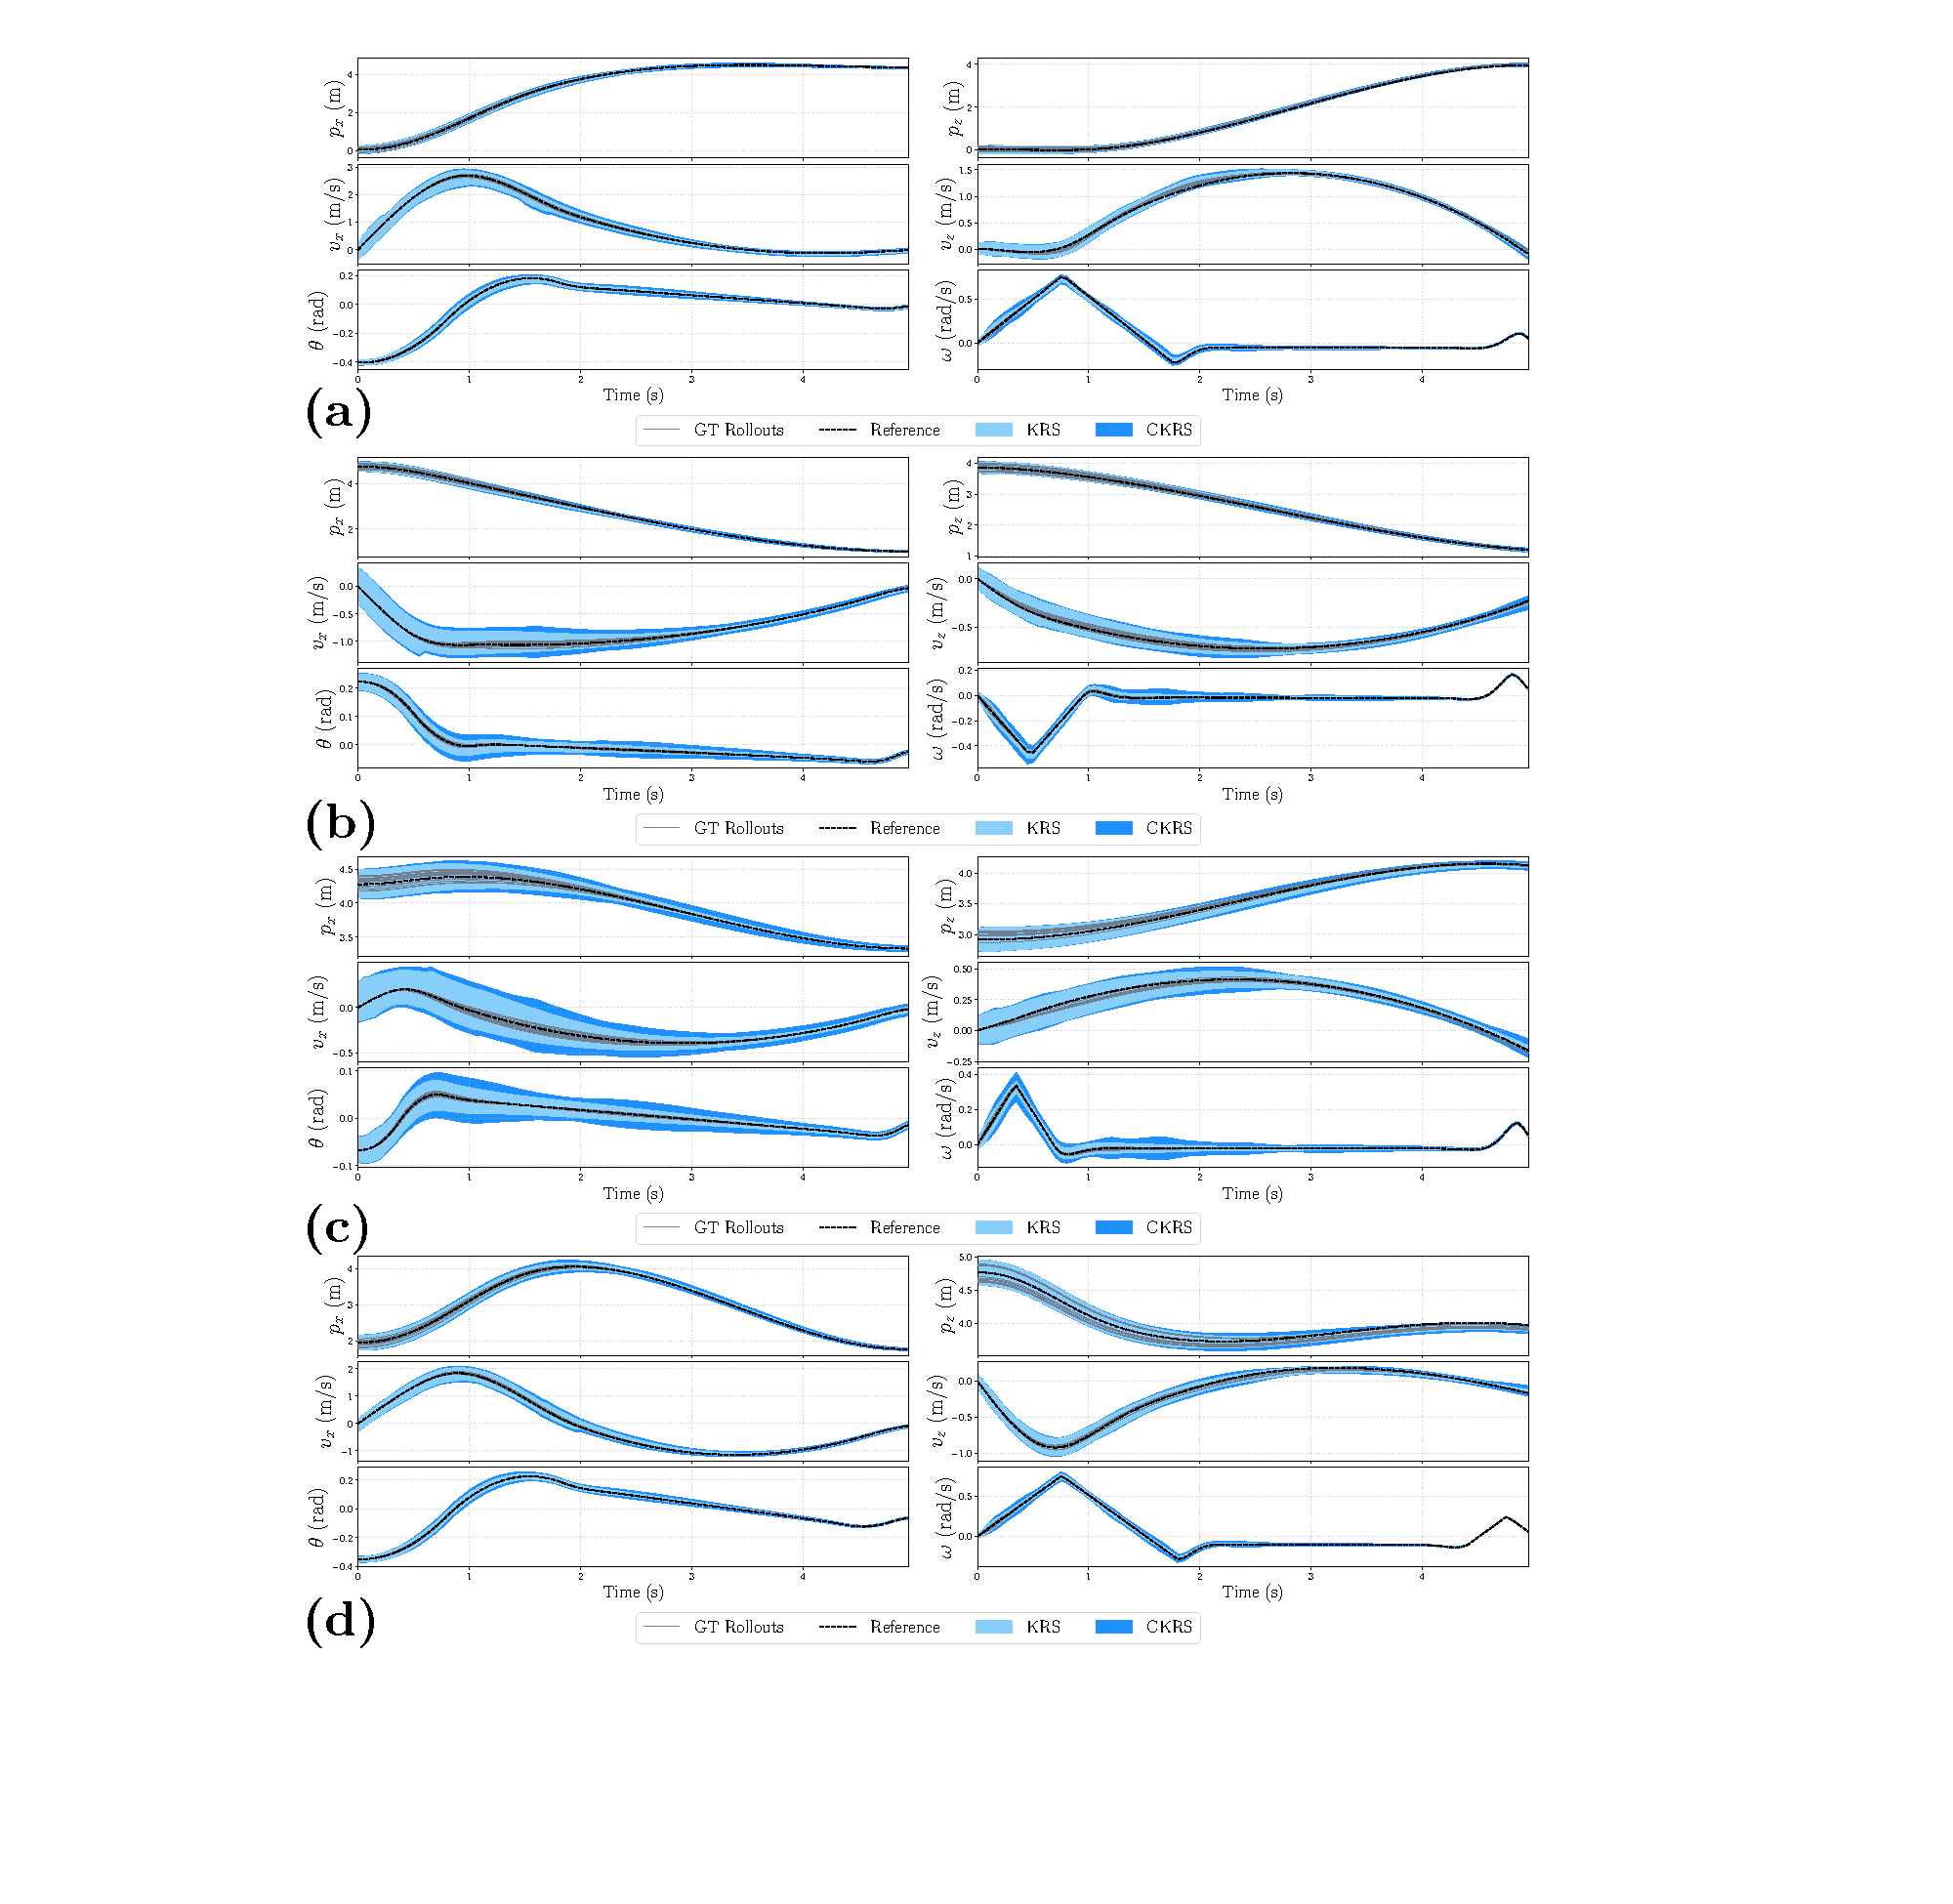
\includegraphics[width=1\linewidth]{img/2dquad/2dquad_offline_all.pdf}%\includegraphics[width=1\linewidth]{img/2dquad/2dquad.pdf}
    \caption{CKRS computed for four reference trajectories on a 2D quadcopter model, with offline-calibrated CP bounds.}
    \label{fig:2d_quad}
% \vspace{-10pt}
\end{figure}

\subsubsection{Additional results on 3D quadrotor system.}\label{app:3d_quad}

To verify that the offline CP inflation bounds (described in Sec. \ref{sec:conformalize_KRS}) generalize across multiple reference trajectories, we compute the CKRS for three alternative reference trajectories and show that the resulting closed-loop trajectories remain within the computed set (Fig. \ref{fig:3d_quad_alt}). This indicates that a single offline CP calibration can be reused to efficiently inflate reachable sets computed online. We also visualize two of these CKRSs together with the obstacle that the quadrotor is navigating around (Fig. \ref{fig:3d_quad_obstacle}), showing that since the RSOAs do not intersect with the obstacle, the closed-loop system is guaranteed to avoid collision when tracking either reference.
\begin{figure}[ht]
    \centering
    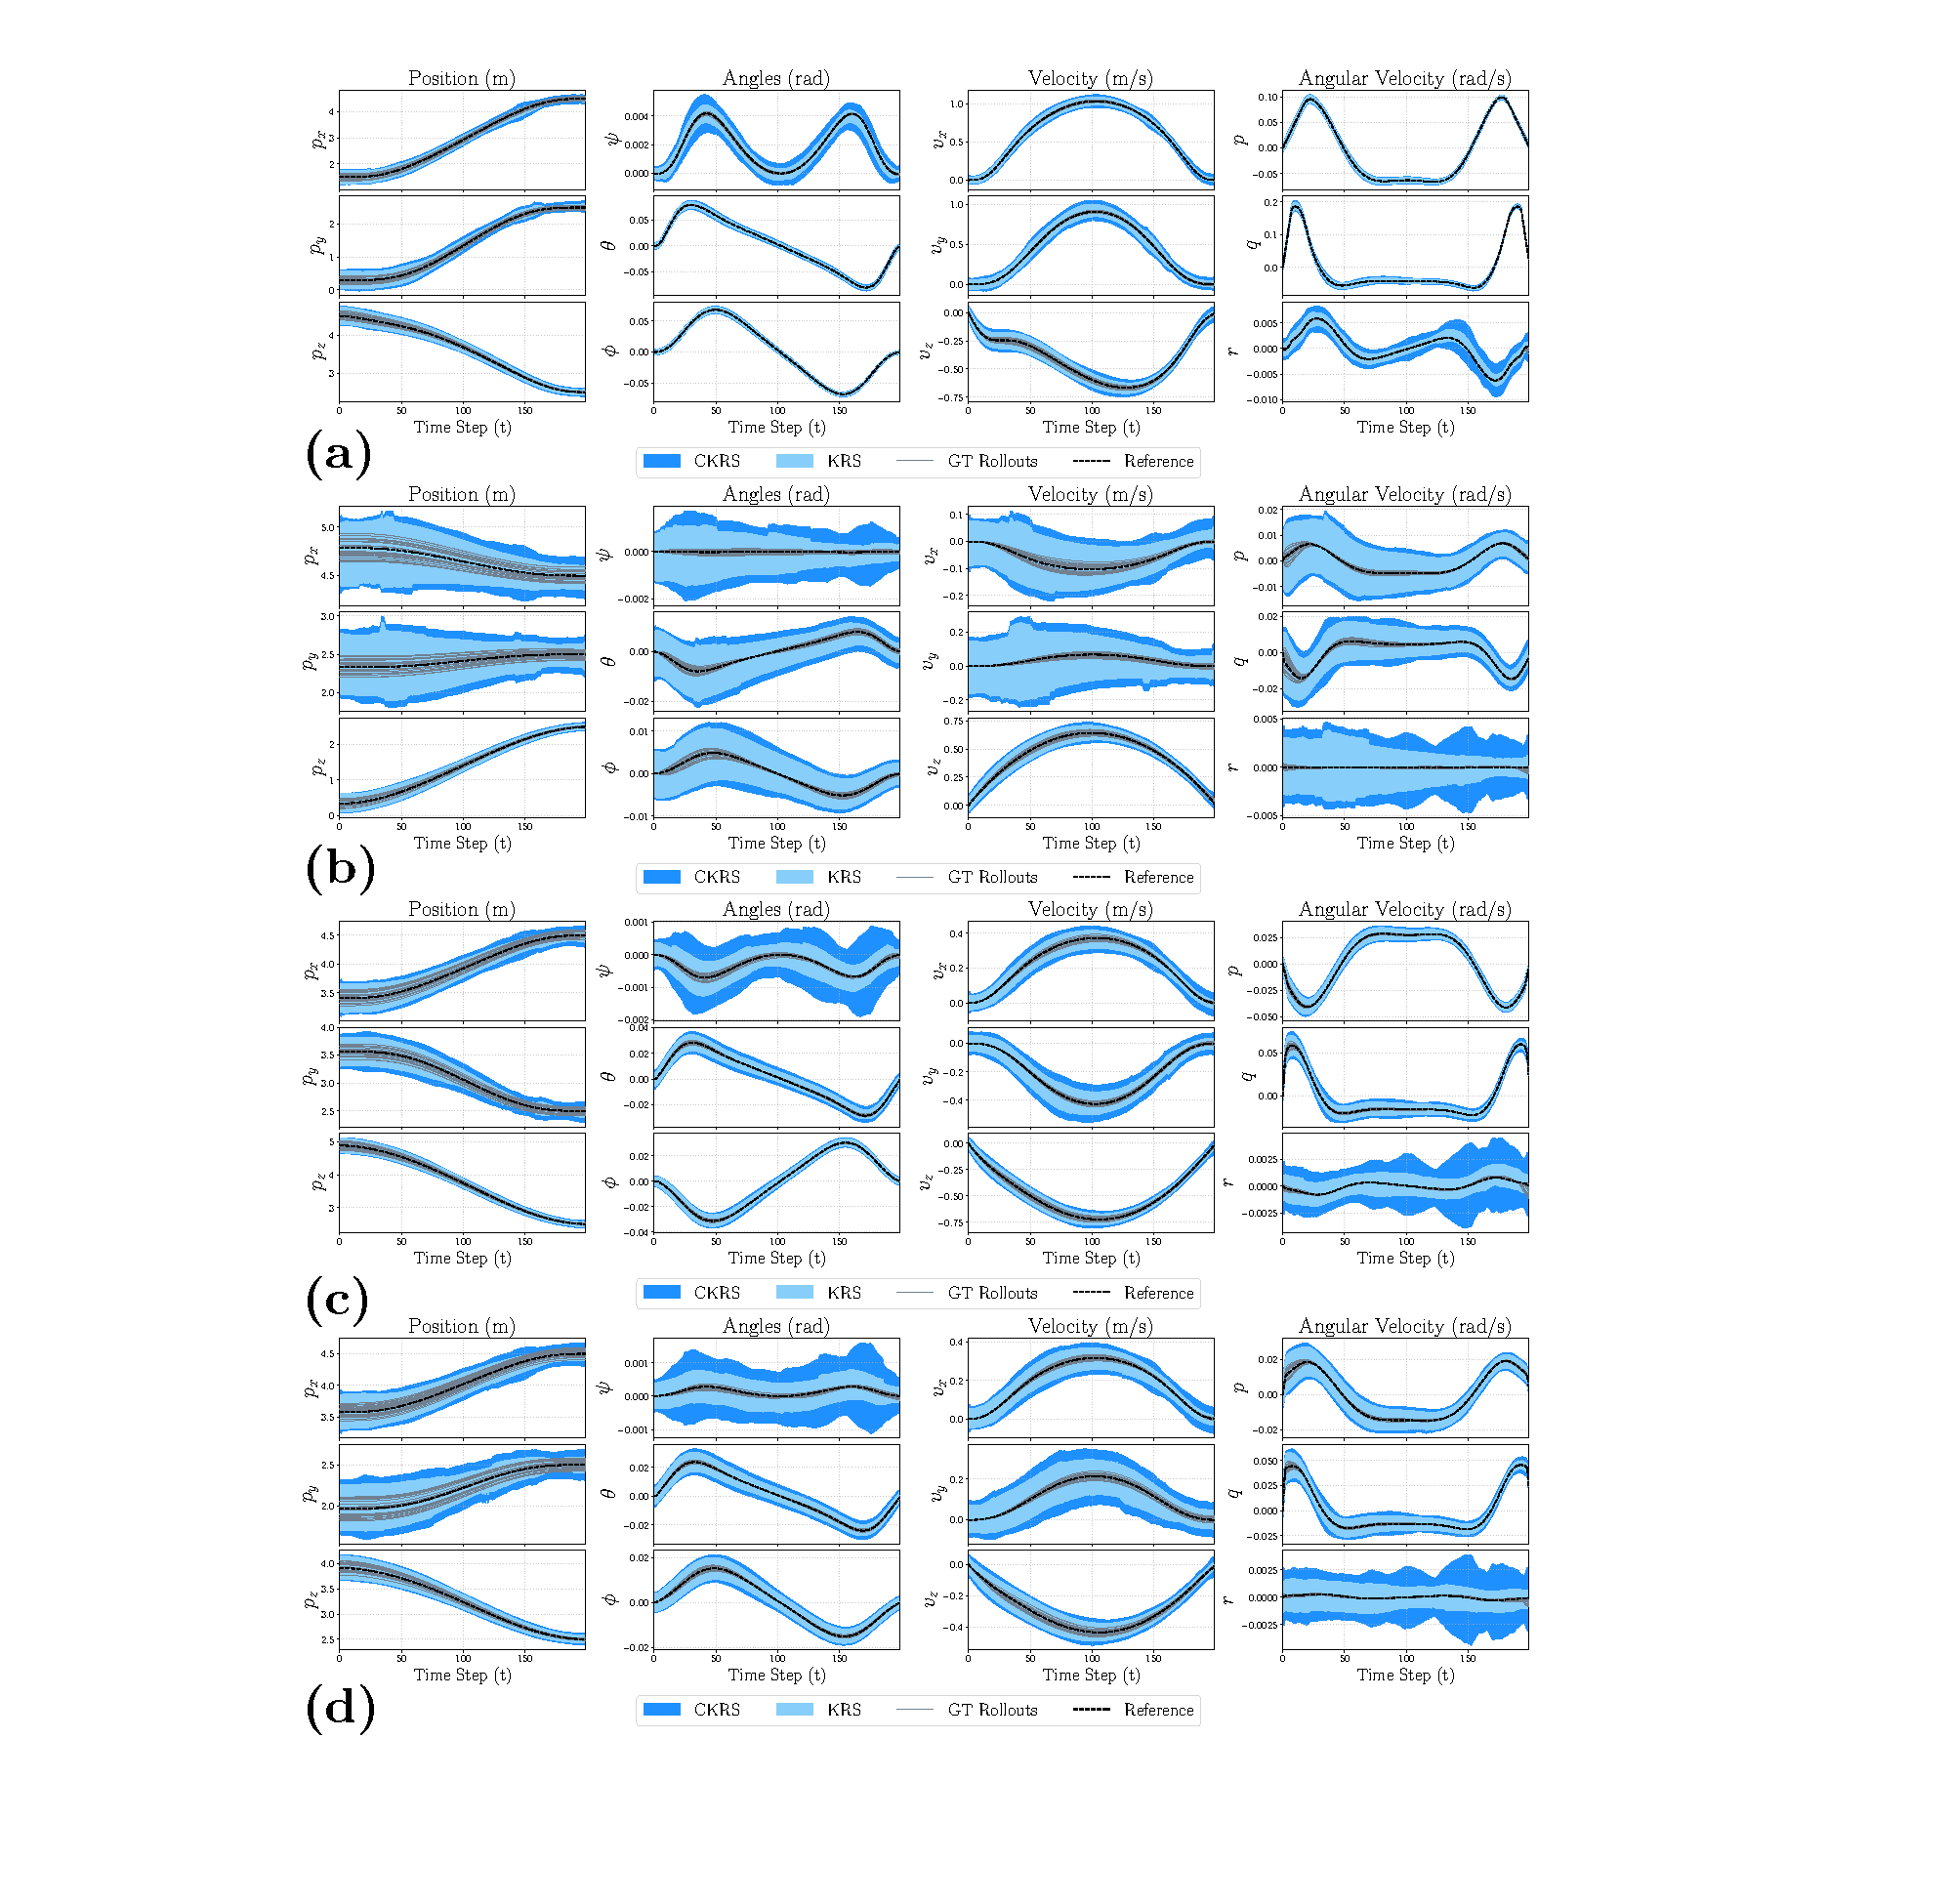
\includegraphics[width=1\linewidth]{img/3dquad/3dquad_offline_all.pdf}%\includegraphics[width=1\linewidth]{img/3dquad/3dquad_alt.pdf}
    \caption{Alternative CKRSs computed for 3D quadcopter model for a different reference trajectory.}
    \label{fig:3d_quad_alt}
% \vspace{-10pt}
\end{figure}
\begin{figure}[ht]
    \centering
    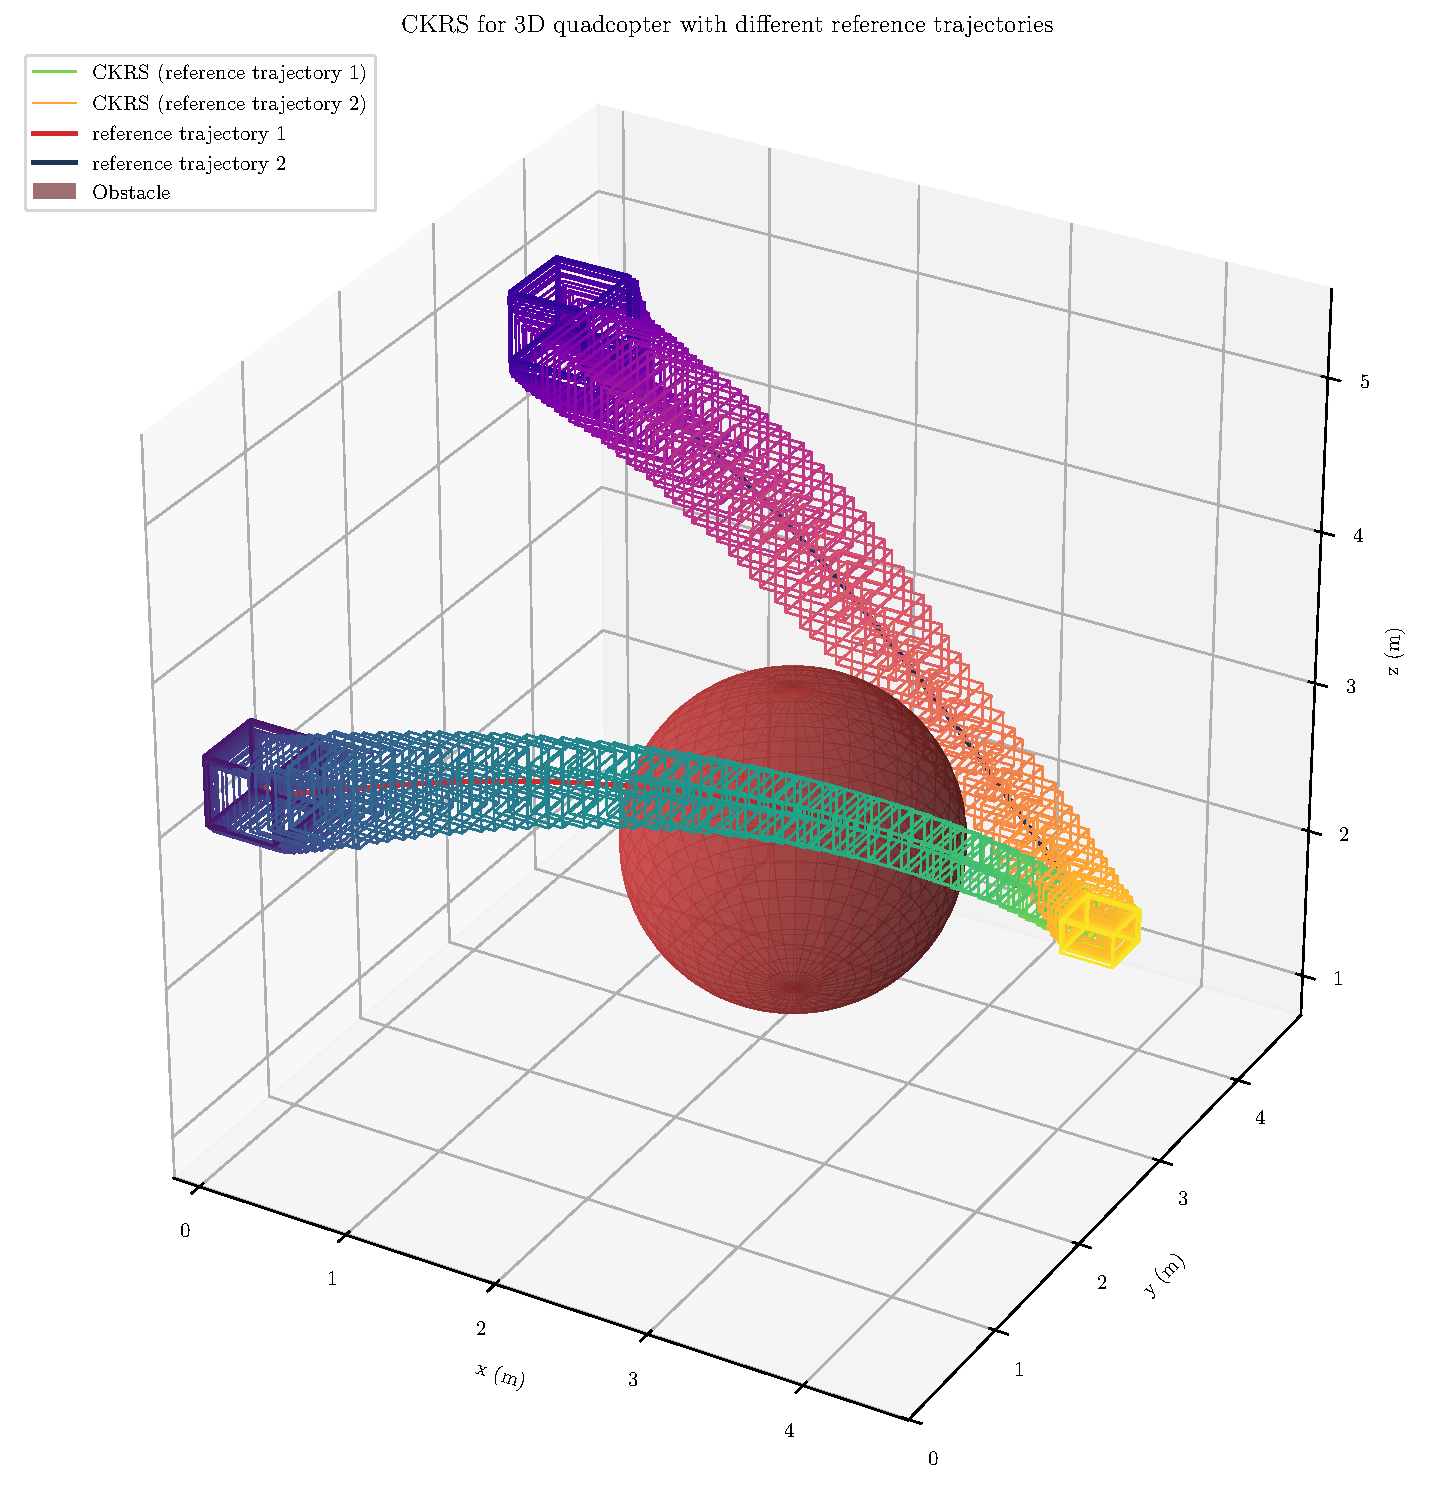
\includegraphics[width=1\linewidth]{img/3dquad/pos_conformal_frs_comparison.pdf}%\includegraphics[width=1\linewidth]{img/3dquad/3dquad_alt.pdf}
    \caption{CKRSs computed for a 3D quadcopter model (position components), overlaid with obstacle.}
    \label{fig:3d_quad_obstacle}
% \vspace{-10pt}
\end{figure}

\subsubsection{Additional results on MuJoCo hopper system.}\label{app:hopper}
Figure~\ref{fig:hopper_exp} illustrates the full state-space evolution of the 11-dimensional MuJoCo Hopper \citep{todorov2012mujoco} system during a forward hopping maneuver. This system poses a unique challenge due to its hybrid dynamics, characterized by non-smooth transitions during ground impacts. The periodic stability of the gait is clearly visible in the ``height z" and ``torso angle" trajectories, where the ScaRe-Kro framework successfully captures the complex dynamics associated with the flight and stance phases. Notably, while the position states exhibit tight confinement around the reference trajectory (dashed black line), the velocity dimensions (e.g., ``Velocity Foot") display a necessary inflation of the conformal bounds. This expansion correctly accounts for the instantaneous jumps in state caused by contact forces and modeling uncertainties at impact, yet the ground truth rollouts remain strictly contained within the predicted tube, validating the robustness of the Koopman tracking controller under discontinuous contact dynamics.

\begin{figure}[ht]
    \centering
    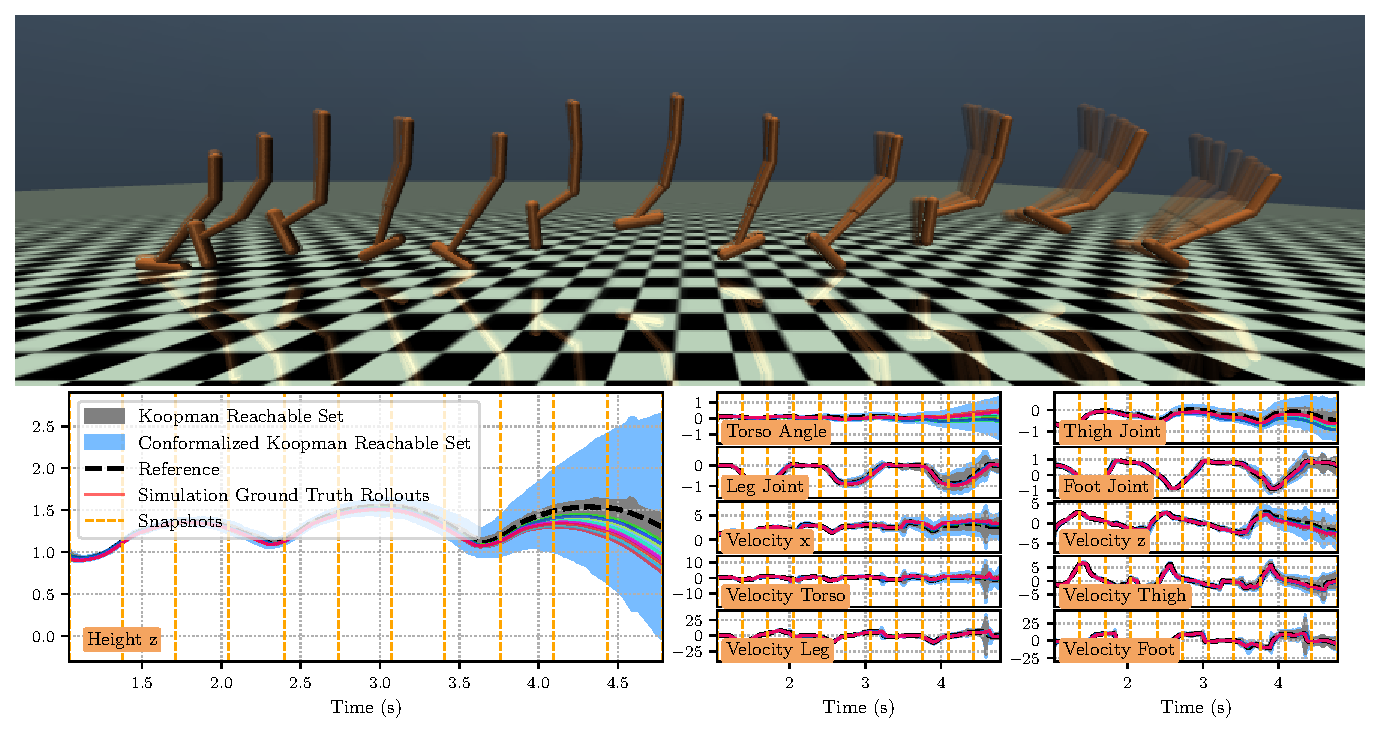
\includegraphics[width=1\linewidth]{img/hopper/Hopper_Fig.pdf}
    \caption{CKRS and KRS computed for 11-D MuJoCo Hopper. The thin multi-colored lines denote distinct closed-loop trajectory rollouts.}
    \label{fig:hopper_exp}
% \vspace{-10pt}
\end{figure}

\subsubsection{Additional results on MuJoCo swimmer system.}\label{app:swimmer}
Figure~\ref{fig:swimmer} presents the component-wise reachability analysis for the 28-dimensional MuJoCo Swimmer \cite{todorov2012mujoco}, representing the most high-dimensional validation of our framework. The plots display the highly coupled, undulatory gait required for locomotion, evidenced by the phase-shifted oscillations across the chain of link joints and velocities. Despite the significant increase in state dimensionality, the CKRS maintain consistent coverage of the closed-loop trajectories across all 28 dimensions. The uniform tightness of the bounds across the swimmer link segments confirms that the learned globally-linear dynamics structure effectively encodes the multi-body dynamics, enabling safe, long-horizon verification for complex, articulated robots while maintaining tractable computation.

\begin{figure}[ht]
    \centering
    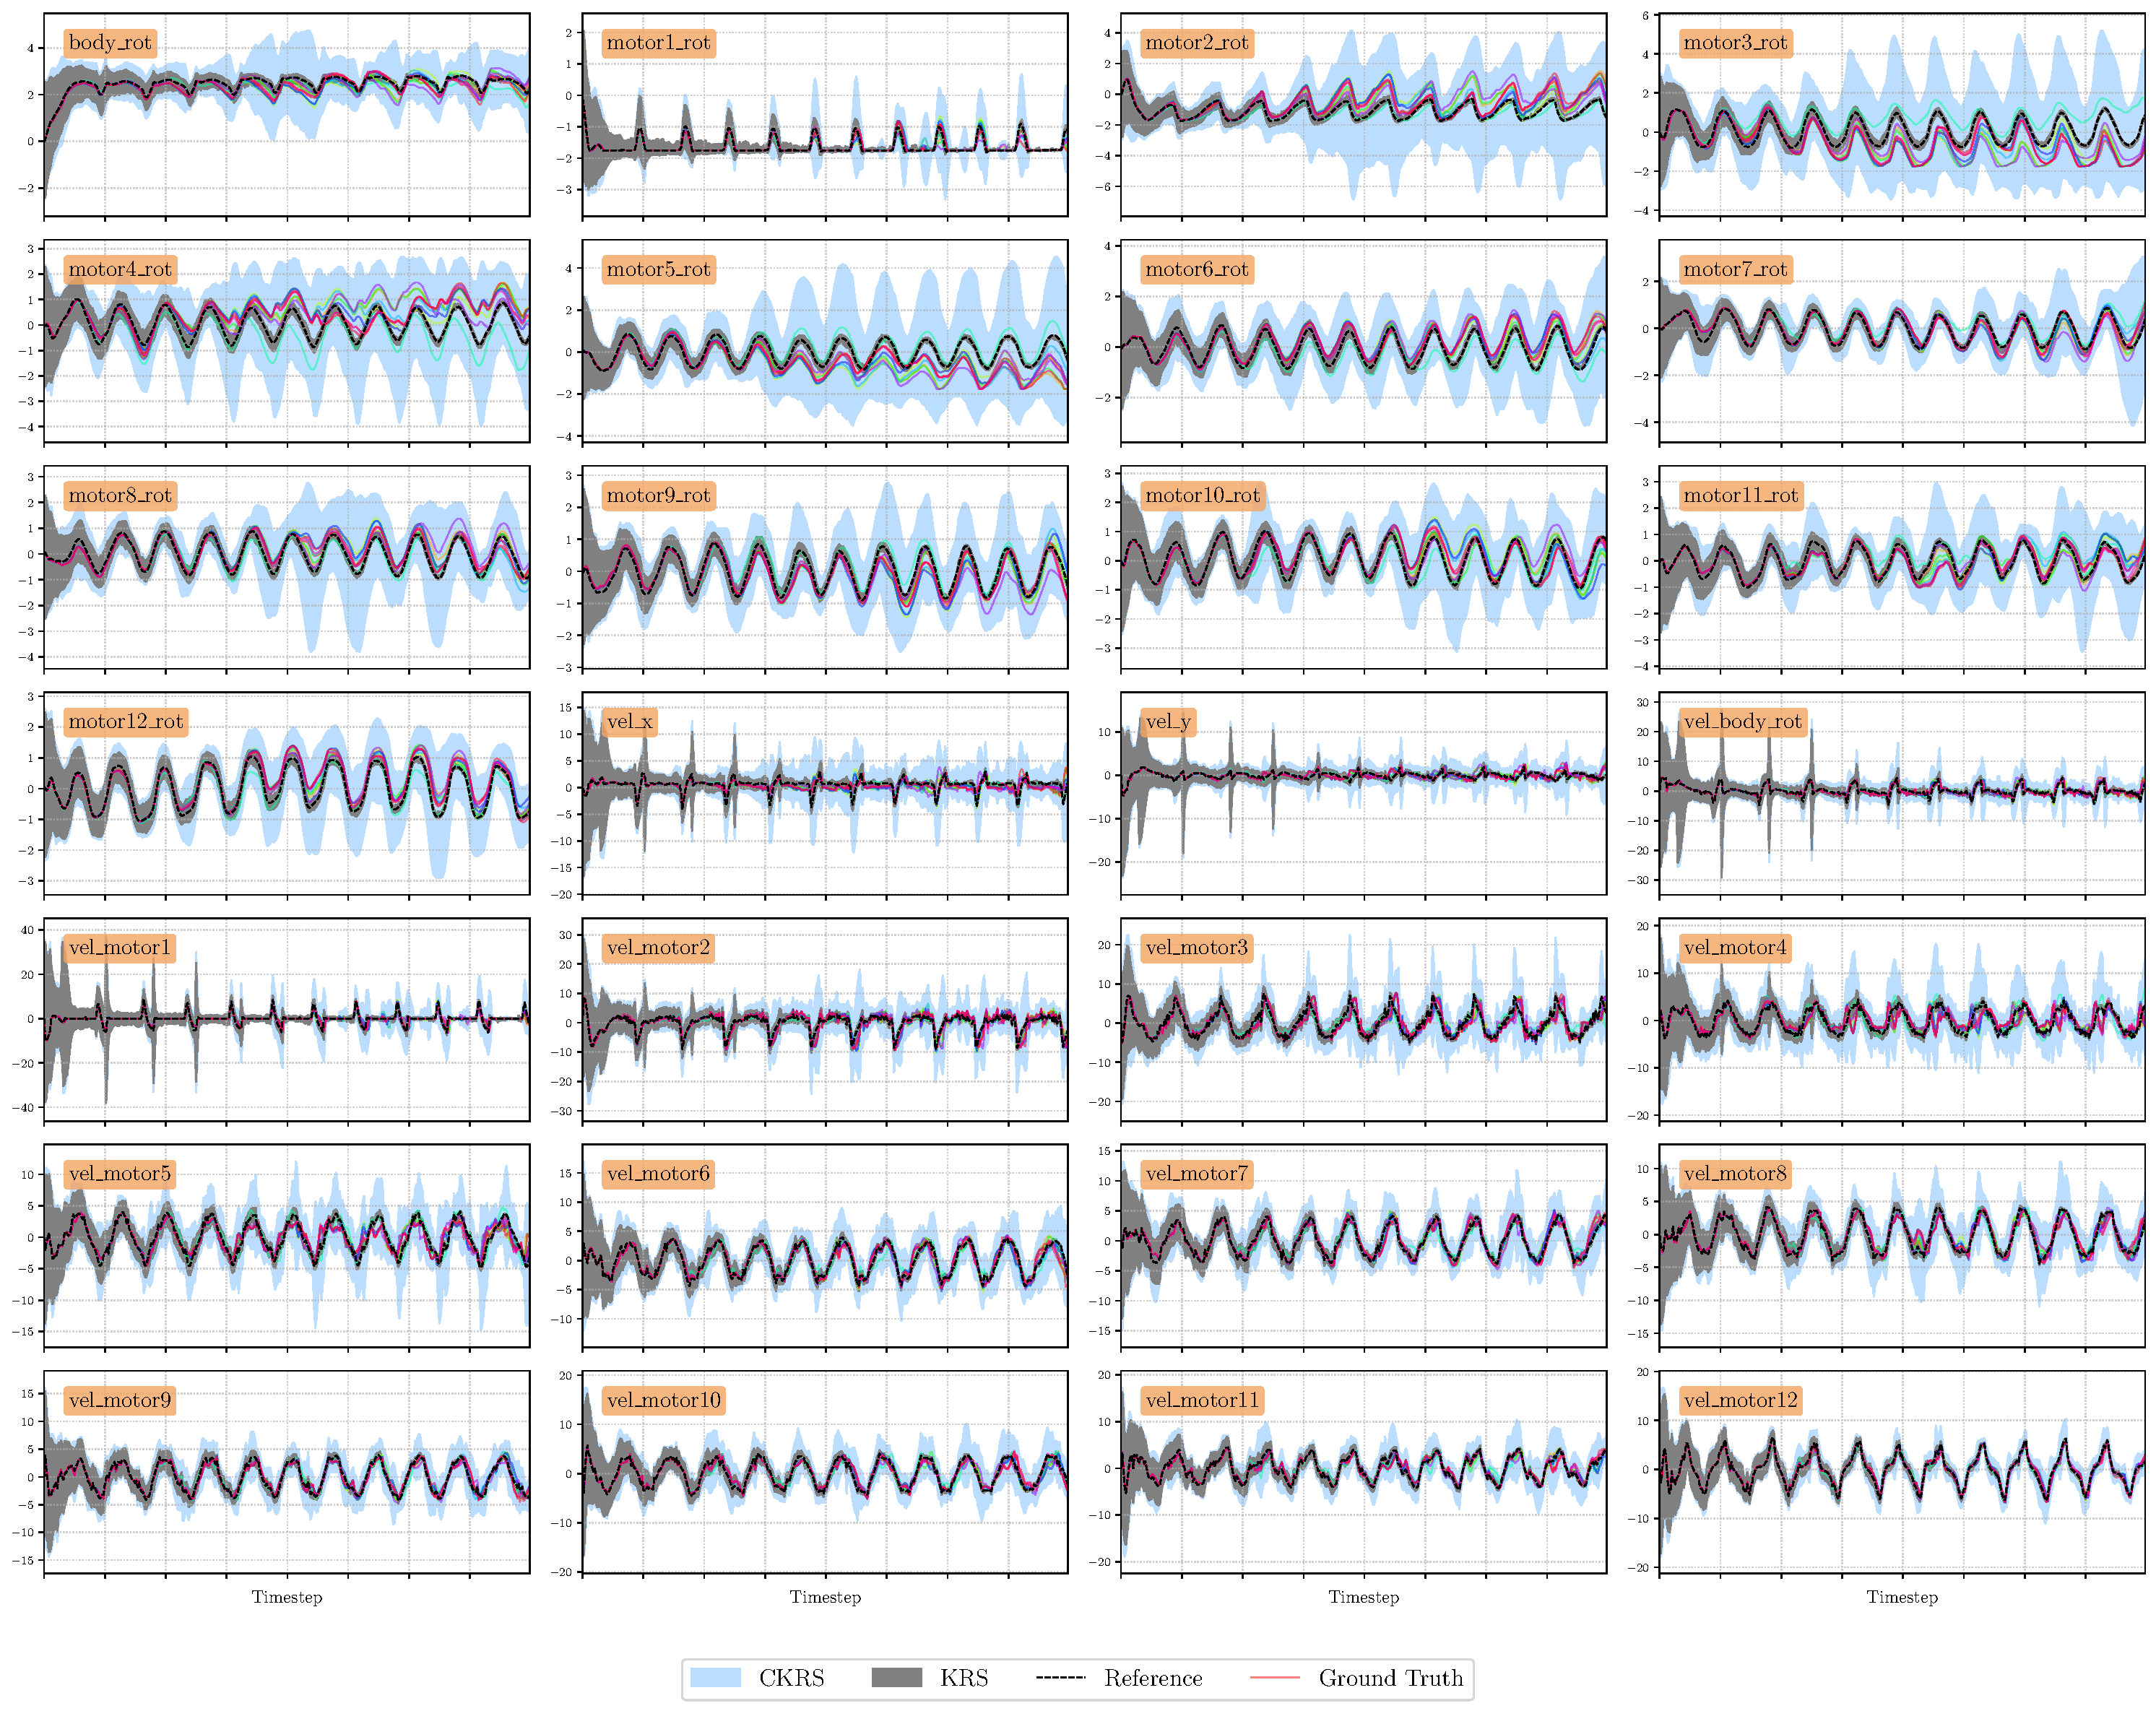
\includegraphics[width=1\linewidth]{img/swimmer/Swimmer_All_States_28D.pdf}
    \caption{CKRS and KRS computed for 28-D MuJoCo Swimmer. The thin multi-colored lines denote distinct closed-loop trajectory rollouts.}
    \label{fig:swimmer}
% \vspace{-10pt}
\end{figure}